\appendix
\appendixpage

\section{Magenta benchmarks results}
\label{appendix:magenta_benchmark}
\begin{minipage}{\linewidth}
    \captionof{table}{Magenta Generalized Benchmark Times (in seconds).}
    \begin{adjustbox}{width=\textwidth}
        \csvautotabular[respect underscore=true]{raspberry_pi_4_magenta.csv}
    \end{adjustbox}
\end{minipage}

\section{Attributions}

\begin{itemize}
    \item \autoref{fig:rpi4b} comes from the Raspberry Pi Foundation and is licensed under the Creative
          Commons Attribution-ShareAlike 4.0 International license. The original can be found at:
          \url{https://projects.raspberrypi.org/en/projects/raspberry-pi-setting-up/1}.

    \item \autoref{fig:rpios} comes from the Raspberry Pi Foundation and is licensed under the Creative
          Commons Attribution-ShareAlike 4.0 International license. The original can be found at:
          \url{https://projects.raspberrypi.org/en/projects/raspberry-pi-setting-up/4}.

    \item \autoref{fig:gpio} comes from the Raspberry Pi Foundation and is licensed under the Creative
          Commons Attribution-ShareAlike 4.0 International license. The original can be found at:
          \url{https://www.raspberrypi.org/documentation/usage/gpio/}.
\end{itemize}

\section{MusicXML format}

MusicXML is a standard format to transfer music data sheets. It is intended to be
automatically parsed. For this reason, the format is not intuitively good for human
reading.

Here is an example of this format to describe a single whole note middle C in C major key
on Treble Clef:

\begin{figure}[h!]
    \centering
    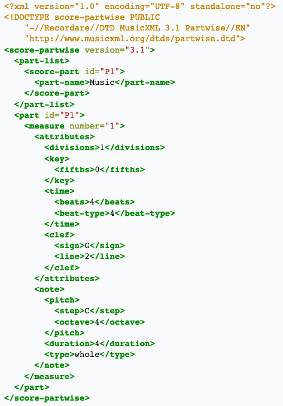
\includegraphics[width=\linewidth]{image/fig_JDF29.png}
\end{figure}

\section{PolyphonyRNN format}

This music representation format is used by the same name model in Magenta library.
Similar to MIDI, represents polyphonic music. Here is an example representing a C major
chord with duration of one quarter per note:

\begin{figure}[h!]
    \caption{Representation of C major chord with duration of one quarter per note}
    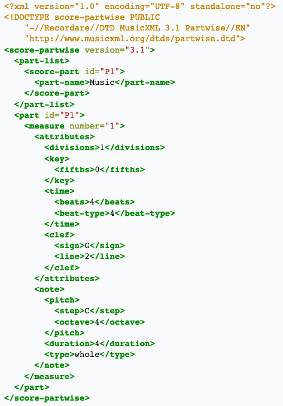
\includegraphics[width=\linewidth]{image/fig_JDF29.png}
\end{figure}


\section{NoteSequences - Protocol Buffers}

This protocol created by Google is a language/platform neutral “extensible mechanism”
(cite Google website https://developers.google.com/protocol-buffers/) for serialization of
structures data. In simple words, this is an equivalent serialization format as is XML or
JSON formats. The added value is that is possible to serialize data in one single format
and Google’s compiler provides the data in the shape of the target language/platform.

The final compiled serialization is in binary format.

\begin{figure}[h!]
    \caption{The final compiled serialization is in binary format.}
    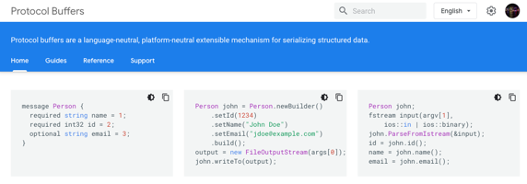
\includegraphics[width=\linewidth]{image/fig_JDF31.png}
\end{figure}

\begin{figure}[h!]
    \caption{The final compiled serialization is in binary format.}
    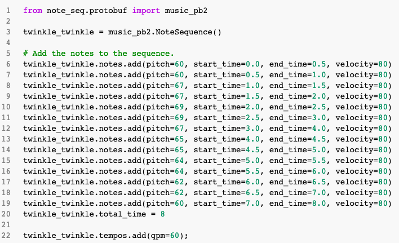
\includegraphics[width=\linewidth]{image/fig_JDF32.png}
\end{figure}

\section{General Flow For Machine Learning Modeling}

Generating machine learning models can seems a huge task. In a sense it is: the variables
in place can produce a virtual infinite universe of possible answers where a few are close
enough to generalize correctly under a specific application. However, some stages are
commonly followed across the practice of modeling. In this section we will try to capture
those generic task as a starting point for any machine learning modeling work.

\begin{enumerate}
    \item Data collection
    \item Data exploration and pre-processing
    \item Feature engineering
    \item Data conversion to framework model input
    \item Model Design
    \item Model Training
    \item Model Evaluation
    \item Model Readjustment
    \item Model Serialization
    \item Model Conversion for Deployment
\end{enumerate}

\newpage